\newcommand\helampl{\mathcal{A}_{\vb*{\lambda}}}

In \cref{chap:stdtech,chap:numunitarity} we were operating on the objects under the assumption that they are Lorentz scalars.
However in QFT scattering amplitudes of particles with spin are not Lorentz scalars,
and the set of all Lorentz structures generated from Feynman diagrams is immensely redundant.
In this chapter we will discuss how amplitudes of any scattering process, 
polarized or not, can be decomposed into a minimal basis of Lorentz-invariant objects.

It is well known that the full physical information about any scattering process is contained in a complete set of \textit{helicity amplitudes} ---
the amplitudes with all external particles' states chosen to have a definite helicity (see the definition in \cref{chap:4dspinhel}).
Being non-redundant and complete representation of physical information, the helicity amplitudes 
enjoy a number of nice properties such as trivialization of gauge-invariance and manifestation of Poincaré symmetry.
On a technical side the consequence is that the helicity amplitudes are expected to have the most compact representation.
And indeed this has been shown to be the case in numerous practical applications (see e.g.\ %
\cite{DeLaurentis:2019phz,Badger:2019djh,Badger:2011yu,Badger:2013gxa,DeFreitas:2004kmi,Gehrmann:2011aa,Gehrmann:2009vu,Glover:2004si,Glover:2003cm,Garland:2002ak,Dunbar:2016aux,Dunbar:2016gjb,Dunbar:2016cxp,Badger:2015lda,Gehrmann:2015bfy,Bern:2003ck,Bern:2002tk,Badger:2018enw,Dunbar2017,Kunszt:1994nq}).

The computation of tree-level helicity amplitudes is a very straight-forward task,
which amounts to simply inserting the corresponding states with definite helicities for each external particle.
The spinor-helicity techniques can be employed to further enhance the computations.
Moving forward to amplitudes with loops,
we are forced to make the dimensionality of space-time formally infinite \cite{Collins:1984xc} 
to regularize divergences.\footnote{other regularization methods are out of the scope of this thesis}
This fact makes both definition and evaluation of helicity amplitudes rather delicate.
It is the purpose of this chapter to present a concise and efficient method of
evaluating multi-loop helicity amplitudes in dimensional regularization,
amenable for numerical applications.

In \cref{sec:helampl_projectors} we briefly review a somewhat standard 
method of obtaining helicity amplitudes through $D$-dimensional projectors,
which can be found in the literature \cite{Garland:2002ak, Moch:2002hm, Glover:2003cm, Glover:2004si,Gehrmann:2009vu,Gehrmann:2011aa}. 
In \cref{sec:helampl_embeding}, 
taking advantage of some insights from \cref{chap:numunitarity},
we show how the tree-level approach of ``simply inserting appropriate external states'' can
be extended to loop amplitudes in the 't Hooft-Veltman (HV) flavor of dimensional regularization.
This allows to dispose of construction of complicated projectors, which
become vary hard to handle for large $(> 4)$ number of particles with spin \cite{Peraro:2019cjj}. 
Another convenient feature of our approach is that it can be applied in a numerical context, such
as evaluation of cuts through off-shell recursion as discussed in \cref{sec:evaluation_of_cuts}.
In \cref{sec:ds_reduction} we discuss how
the efficiency of extraction of the full $D_s$-dependence can be substantially improved
by dimensionally reducing kinematically-independent degrees of freedom in higher dimensions.

\todo{reference spinning particles paper (was for 5 gluon) and another from the guy from MPP} 


\section{Helicity Amplitudes}

A helicity amplitude $\helampl$
is defined as an $\mathcal{S}$-matrix element
with external polarization states $\varepsilon_{i}$ chosen to be
helicity eigenstates (for the definition of helicity see \cref{chap:4dspinhel}) with helicities $\vb*{\lambda}=\{\lambda_1,\ldots{},\lambda_N\}$.
Cross-sections obtained from $\Abs{\helampl{}}$ describe
the scattering of polarized particles.
Unpolarized cross-sections can be obtained by summing over the helicities of all external particles
with the help of the completeness relations
\begin{subequations}
  \label{eq:4d_completeness_relations}
  \begin{align}
    \sum_{\lambda=\{+1,-1\}} \varepsilon^\mu_\lambda(p){\varepsilon^\nu_\lambda}^{\star{}}(p)  &= -g^{\mu\nu} + \frac{p^\mu \eta^\nu + p^\nu \eta^\mu}{\sp(p,\eta)}, \\
    \sum_{\lambda=\{+\frac{1}{2},-\frac{1}{2}\}} u^\alpha_\lambda(p){\overline{u}_\lambda^\beta}(p)  &= \qty(\slashed{p}  \pm m\,\mathbb{1})^{\alpha\beta},
  \end{align}
\end{subequations}
for gauge bosons and fermions correspondingly.
The number of $N$-particle helicity amplitudes is thus $2^N$, and
it can be further reduced by taking into an account charge and parity transformations.

The transformation of helicity amplitudes under the Lorentz boosts is completely specified by their 
external states, and is given by the \emph{little group scaling},
\begin{equation}
  \ket{p_i} \to t_i \ket{p_i}, \quad  \sket{p_i} \to \frac{1}{t_i} \ket{p_i} \implies \helampl \to  \qty(\prod_i t_i^{-2\lambda_i}) \helampl,
\end{equation}
where $t_i$ are complex phases.
As expected the squared matrix element $\Abs{\helampl{}}$ is Lorentz-invariant.
With the help of spinor-helicity formalism we can also make any helicity amplitude itself into a scalar
by removing it's \emph{spinor weight} --- a factor which has the same little group scaling
as the helicity amplitude.
Hence the scalar objects we were operating on in \cref{chap:stdtech,chap:dshel} can be the rescaled helicity amplitudes.

We can perturbatively expand helicity amplitudes in the coupling constants as
\begin{equation}
  \helampl =  \helampl^{(0)} + g^2 \helampl^{(1)} + g^4 \helampl^{(2)} + \ldots{},
\end{equation}
with all leading-order couplings absorbed into $\helampl^{(0)}$.
It is then convenient to use the tree helicity amplitude\footnote{if it is not vanishing} $\helampl ^{(0)}$ to remove the spinor weight
of loop amplitudes.
It should be noted that the definition of helicity amplitudes may not depend on a regularization scheme
used to regularize divergences of loop amplitudes. This implies, that 
among the flavors of dimensional regularization only in the ones which consider external particles 
to be in four dimensions the helicity amplitudes can be consistently defined.

%This can be achieved for example by normalizing all amplitudes $A^{L}_N$ with $L\geq1$ by
%a corresponding tree amplitude $A^{0}_N$ 

\section{Form-Factor Decomposition and Projectors}
\label{sec:helampl_projectors}

In this section we review the conceptually simplest way to define helicity amplitudes in dimensional regularization, which is through $D$-dimensional projectors.
This approach has been used in a number of computations \cite{Garland:2002ak, Moch:2002hm, Glover:2003cm, Glover:2004si,Gehrmann:2009vu,Gehrmann:2011aa}.
It's relation to HV scheme and helicity amplitudes has been recently clarified in \cite{Peraro:2019cjj} (see also \cite{Chen:2019wyb}).

One starts with decomposing an amplitude with \emph{unspecified} external states into all possible $D$-dimensional tensor structures $\mathcal{T}_i$ compatible
with symmetries and gauge invariance,
\begin{equation}
  \mathcal{A}  = \sum_{i} \mathcal{T}_i\;A_i.
\end{equation}
For example $\mathcal{T}_i$ can contain object like $\sp(\varepsilon(p_i),p_j)$, $\bar{v}(p_i) \slashed{p}_j u(p_k) $, $\bar{u}(p_i) \slashed{\varepsilon}(p_j) u(p_k)$, etc.
Here $A_i$ are the Lorentz-invariant form-factors.
Then one finds projectors $\mathcal{P}_i$ on $A_i$ from linear combinations of $\mathcal{T}_i$ by solving the equations
\begin{equation} \label{eq:cdr_projectors}
  \mathcal{P}_i [\mathcal{A}] = \qty(\sum_j c_{i,j}(\vb*{x},D) \sum_\text{(states)} \mathcal{T}^{\dagger}_j) \qty[\sum_{k} \mathcal{T}_k A_k] = A_i, 
\end{equation}
for the coefficients $c_{i,j}(\vb*{x},D)$, which are rational functions of external kinematics $\vb*{x}$ and $D$.
Here the state sums are taken to be in $D$ dimensions, which corresponds to working in the CDR scheme.

To extract the helicity amplitudes one then \textit{evaluates} the tensor structures $\mathcal{T}_i$ 
by inserting the corresponding \textit{helicity states in four dimensions} for each of the external particles. 
This is equivalent to switching to the HV scheme.
The procedure uncovers the fact that only particular linear combinations of $A_i$ are relevant,
and the number of these combinations is exactly the number of independent helicity amplitudes, which is
significantly lower than the number of initial tensor structures $\mathcal{T}_i$.

The difficulties of this approach are two-fold:
\begin{enumerate}
  \item The number of initial tensor structures grows very fast with the number of external particles with spin.
    This makes solving the equations \cref{eq:cdr_projectors} for projectors and then applying them to each Feynman diagram very challenging for $N>4$.
  \item The projectors have to be applied to analytic expressions since the external states in $D$ dimensions do not admit any finite numerical representations \cite{Collins:1984xc}.
\end{enumerate}

Since the helicity amplitudes contain the complete physical information, 
the construction of form-factors in  \cref{eq:cdr_projectors} seems to be an unnecessary complication.
And indeed a way to avoid these steps and construct the projector onto helicity amplitudes directly has been suggested recently \cite{Peraro:2019cjj}.
This somewhat mitigates the first issue, but the projectors have to be still applied to analytic expressions.

\section{Helicity Amplitudes in the HV Scheme from Embedding of States}
\label{sec:helampl_embeding}

In this section we explain how multi-loop helicity amplitudes
with vector and spinor external particles can be obtained in dimensional regularization
from appropriate embedding of helicity states into spaces of higher dimensionality $\mathsf{S}_{[D_s]}$.
As in \cref{sec:evaluation_of_cuts}, in this \namecref{chap:dshel} we will denote the dimensionality of particles'
representations as $D_s$.

\todo{
  We build up independently from the projector approach, in the context of dimensional reconstruction. 
  However the correspondence can be straightforwardly established
}

In HV the space-time symmetry group is extended to $\mathrm{SO}(1,D_s-1)$, and the external particles are kept in four dimensions. 
More precisely this means that, like in CDR, the tensor and Clifford algebras are performed in $D_s$ dimensions,
but the completeness relations for external states have to be as in \cref{eq:4d_completeness_relations}. 
In other words the amplitudes in HV transform like their four-dimensional counterpart under $\mathrm{SO}(1,3)$, 
and are invariant under the rotations in $\mathrm{SO}(D_s-4)$. 
This implies that, upon normalizing by an appropriate spinor weight, the helicity amplitudes are scalars of the extended symmetry group $\mathrm{SO}(1,D_s-1)$.
In \cref{chap:numunitarity} we argued that we can use this symmetry to embed the formally infinite-dimensional computation
into a finite one with appropriately chosen integer values of $D^{(L)}$ and $D_s$.
This fact motivates our strategy:
\begin{enumerate}
  \item Consider amplitudes in arbitrary (integer) $D_s > D^{(L)}$ dimensions with fixed external states,
    which have the right little-group behavior with respect to $\mathrm{SO}(1,3) \subset \mathrm{SO}(1,D_s-1)$.
  \item Impose the rotational symmetry in $\mathrm{SO}(D_s-4)$ by combining the degrees of freedom from $\mathsf{S}_{[D_s-4]}$ in
    a suitable way.
  \item Set $D_s\to D$ in the amplitudes obtained from the previous step (which are polynomials in $D_s$).
\end{enumerate}
As we will see shortly, the second step is trivial for vector particles. For fermionic
particles it requires a tensor decomposition similar to the one we discussed in \cref{sec:helampl_projectors},
but enormously simplified by the fact that the indices in  $\mathsf{S}_{[D_s-4]}$ are completely decoupled from kinematics\footnote{
  this applies after the loop integrations are performed, 
  but we can always pull the corresponding projectors into the integrand given that $D_s$ was not set to $D$ yet.
}
and that we can ignore all vector particles.



\subsection{Embedding of Vector States}
\label{sec:embedding_vectors}

Consider the amplitudes for the scattering of massless vector particles.
There are $(D_s - 2)$ states for each particle in $D_s$ dimensions. 
The corresponding polarization sum for a particle with momentum $p$ is 
\begin{equation}
  \sum_{j=1}^{D_s-2} \varepsilon^\mu_j(p){\varepsilon^\nu_j}^{\star{}}(p) = -g_{[4]}^{\mu\nu} + \frac{p^\mu \eta^\nu + p^\nu \eta^\mu}{\sp(p,\eta)} \;-\; g_{[D_s-4]}^{\mu\nu}, 
\end{equation}
where we used $p \in \mathsf{S}_{[4]}$
to make the $(D_s-4)$-dimensional part explicit.
Comparing this to \cref{eq:4d_completeness_relations} we see that we can embed the helicity states as
\begin{align}
  \varepsilon_{1,2}^\mu =
    \begin{dcases}
      \varepsilon^\mu_{+,-}, & \mu\in \mathsf{S}_{[4]},\\
      0, & \mu\in \mathsf{S}_{[D_s-4]},\\
    \end{dcases}
    &&
  \varepsilon_{j}^\mu = \delta^{(j+2)}_\mu, \qfor j\geq 3,
\end{align}
Thus the amplitudes in $D_s$ dimensions with $\varepsilon_{1,2}^\mu$ as external states satisfy the correct little-group scaling trivially.
If we now also take into an account the orthogonality relations 
\begin{align}
  g_{[D_s]}^{\mu\nu} = g^{\mu\nu}_{[4]}+g^{\mu\nu}_{[D_s-4]}, && (g_{[4]})^{\mu\rho}(g_{[D_s-4]})_{\rho\nu} = 0,
      %& (g_{[x]})^{\mu}_\mu =x, \qfor x \in  \{4,D_s,D_s-4\},
\end{align}
we see that these amplitudes are invariants under the rotations in $\mathsf{S}_{[D_s-4]}$.
Hence they are the helicity amplitudes in the HV scheme.
This is, of course, a well-known fact which has been exploited in one-loop computations with numerical generalized
unitary methods \cite{Ellis:2007br,Giele:2008ve}, as well as as 
in the so-called six-dimensional helicity formalism \cite{Bern2011,Cheung:2009dc,Badger:2013gxa,Badger:2017jhb}.

Note that, in contrast to the form-factor decomposition in \cref{sec:helampl_projectors}, we did not need any projectors.

\subsection{Embedding of Spinor States}
\label{sec:embedding_spinors}

We now consider amplitudes with external fermions.
There are $2^{\frac{D_s}{2}-1}$ spinor states in $D_s$ dimensions, 
which can be constructed through the representations of Clifford algebras (see \cref{sec:clifford_algebra_ds}).
The polarization sum with the momentum $p \in \mathsf{S}_{[4]}$ is
\begin{equation}
  \sum_{j=1}^{2^{\frac{D_s}{2}-1}} u^\alpha_j(p){\overline{u}_j^\beta}(p) = \qty(\slashed{p}_{[D_s]}  \pm m\,\mathbb{1}_{[D_s]})^{\alpha\beta} \equiv 
  \qty(\slashed{p}_{[4]} \pm m \cdot \mathbb{1}_{[4]})^{\bar{\alpha}\bar{\beta}} \qty(\mathbb{1}_{[D_s-4]})^{\hat{a}\hat{b}},
\end{equation}
where the indices $\alpha = \bar{\alpha}\otimes\hat{\alpha}$,  $\beta = \bar{\beta}\otimes \hat{\beta}$ are factorized into 
$\{\bar{\alpha},\bar{\beta}\}\in \mathsf{S}_{[4]}$ and $\{\hat{\alpha},\hat{\beta}\}\in \mathsf{S}_{[D_s-4]}$.
Comparing to \cref{eq:4d_completeness_relations}, we see that we can embed the four-dimensional spinors as
\begin{align} \label{eq:fermionicStates}
    \qty(u_{\lambda,i})^{\bar{\alpha}\hat{\alpha}} =  u_{\lambda}^{\bar{\alpha}} \cdot \delta_i^{\hat{\alpha}}, && i = 1,\ldots{},2^{\frac{D_s}{2}-2},
\end{align}
where we replaced the index $j \to \{\lambda, i \}$ to make the four-dimensional helicity $\lambda \in  \{+\frac{1}{2},-\frac{1}{2}\}$ manifest.
Thus the amplitudes in $D_s$ dimensions with any of the spinors $\qty(u_{\lambda,i})^{\bar{\alpha}\hat{\alpha}}$ taken as external fermionic states\footnote{
  The fact the these spinors also satisfy the Dirac equation in $D_s$ dimension can be easily verified.
}
(and with the vector states taken as in \cref{sec:embedding_vectors}) have the correct little-group scaling.
However, as opposed to the case of vector particles, we observe that 
all of the states in \cref{eq:fermionicStates} introduce a \emph{preferred direction} in  $\mathsf{S}_{[D_s-4]}$
via the indices $\hat{\alpha}$.
Hence the corresponding amplitudes are \textbf{not} symmetric under the rotations $\mathrm{SO}(D_s-4)$.
From a different point of view, we have many states with the same helicity, which creates an ambiguity as to what 
should be the helicity amplitude.
On that account, we turn to the tensor decomposition of indices $\hat{\alpha}$.

\subsection{Tensor Decomposition in $D_s-4$}
\label{sec:HelAmplHV}

We decompose an amplitude with external fermions in $D_s$ dimensions as
\begin{equation} \label{eq:tensorDecomposition}
  \mathcal{A} = \sum_n v_n A_n,
\end{equation}
where all spinor indices $\hat{\alpha}_i \in \mathsf{S}_{[D_s-4]}$ (and only them) are absorbed into $v_n$,
and, consequently, $A_n$ are scalars of $\mathsf{S}_{[D_s-4]}$.
In the following we will show how to construct a convenient basis of the tensor structures $v_n$ 
for any number of external fermions.

First we observe that only the spinor chains of the form
\begin{equation}
  u^{\hat{\alpha}}_i \; \qty( \prod_k \gamma^{\mu_k}_{[D_s -4 ]} )^{\hat{\alpha}\hat{\beta}} \; u^{\hat{\beta}}_j \quad\equiv\quad 
  \qty( \prod_k \gamma^{\mu_k}_{[D_s -4 ]} )^{i j},
\end{equation}
with indices $\mu_i \in \mathsf{S}_{[D_s -4]}$ contracted to other spinor chains, contribute to $v_n$.
This is the consequence of the following facts:
\begin{itemize}
  \item Thanks to our choice of states for vector particles, all Lorentz vectors that can be contracted with $\gamma^{\mu_i}_{[D_s]}$
    project them into $\mathsf{S}_{[4]}$:
    \begin{align} \label{eq:trivialTens1}
      a_{\mu}
      \left( \gamma_{[D_s]}^\mu \right)_{\bar{\alpha}\hat{\alpha}}^{\bar{\beta}\hat{\beta}} =
      a_{\mu}\left(\gamma_{[4]}^\mu \right)_{\bar{\alpha}}^{\bar{\beta}} \delta_{\hat{\alpha}}^{\hat{\beta}}\,,
      &&
      a \in \{p_i,\varepsilon_{1,2}(p_i)\}
    \end{align}
  \item Any Lorentz indices inside the same spinor chain can be contracted yielding  
    \begin{equation} \label{eq:trivialTens2}
      \left(\gamma_{[D_s]}^\mu\right)_{\bar{\alpha}\hat{\alpha}}^{\bar{\kappa}\hat{\kappa}}
      \left(\gamma_{[D_s]\mu}^{\phantom{\mu}}\right)_{\bar{\kappa}\hat{\kappa}}^{\bar{\beta}\hat{\beta}}
      =D_s~\delta_{\bar{\alpha}}^{\bar{\beta}}\delta_{\hat{\alpha}}^{\hat{\beta}}\,.
    \end{equation} 
  \item Due to the factorized representation of the Clifford algebra (see \cref{eqn:cliffordrecursion}),
    any spinor chain can be factorized.
\end{itemize}
Non-trivial tensors $v_n$ are thus obtained by contracting
Lorentz indices of multiple chains of $\gamma_{[D_s-4]}$ matrices.
Some examples of $v_n$ are
\begin{equation}
  \begin{aligned}
    & \delta^{i_1}_{j_1} \delta^{i_2}_{j_2},\\
    & (\gamma_{[D_s-4]}^{\mu_1} )_{i_1}^{j_1} (\gamma_{[D_s-4]\mu_1}^{\phantom{\mu}})_{i_2}^{j_2}, \\
    & (\gamma_{\mu_1[D_s-4]}^{\phantom{\mu}} )_{i_1}^{j_1} (\gamma_{[D_s-4]}^{\mu_1}\gamma_{[D_s-4]}^{\mu_2} )_{i_2}^{j_2} (\gamma_{[D_s-4]\mu_2}^{\phantom{\mu}})_{i_3}^{j_3},\\
    & \qquad \vdots{}
  \end{aligned}
\end{equation}

Evidently to construct a basis of tensor structures $v_n$ we can
decompose each of the spinor chains 
into the standard set of antisymmetric (see e.g.\ \cite{Veltman:1988au}) 
\begin{align}\label{eq:basisGammaChainDs}
\gamma_{[D_s-4]}^{\mu_1 \ldots \mu_n} = \frac{1}{n!} \sum_{ \sigma\in S_n} \sgn(\sigma) \gamma_{[D_s-4]}^{\mu_{\sigma(1)}} \ldots \gamma_{[D_s-4]}^{\mu_{\sigma(n)}}\,,
\end{align}
where $S_n$ denotes the set of all permutations of $n$
integers and $\sgn(\sigma)$ the signature of the permutation
$\sigma\in S_n$.

In practical calculations, one is interested in computing
specific coefficients $M^{(k)}_n$ in the decomposition
of eq.~\eqref{eq:tensorDecomposition}. We construct the
basis $\{v_n\}$ such that this operation is trivial, i.e.\  it
satisfies
\begin{equation}\label{eqn:vnproducts}
	v_n^\dagger\cdot v_m=c_n\delta^n_m\,,
	\quad
    c_0(D_s) = 1\,\quad\mbox{and}\quad  c_{n>0}(D_s)={\cal O}(\epsilon)\,.
\end{equation}
The calculation of the coefficients $c_n$ requires some 
technical operations on $\gamma$ matrices that we present in
appendix~\ref{sec:identities}.
We then construct the dual basis $\{v^n\}$, with elements
\begin{equation}\label{eq:dualBasis}
	v^n=\frac{1}{c_n} (v_n)^\dagger\,.
\end{equation}
Using the dual basis, we directly get
\begin{equation}\label{eqn:helampl}
  M^{(k)}_n = v^n \cdot M^{(k)}.
\end{equation}


\subsubsection{Examples}

As a first and trivial example let us consider an amplitude with a pair $q\bar q$ of external
quarks and any number of external gluons. There is a single
chain of $\gamma_{[D_s-4]}$ matrices and, as there are no other objects with $(D_s-4)$ indices,
for this case there is only a single term in the decomposition in \cref{eq:tensorDecomposition}:
\begin{equation}\label{eq:decompqqbar}
  \mathcal{A}(q,\bar q,g,\ldots,g) =v_0\,A_0\,,\qquad \textrm{with}\quad (v_0)_{\hat{\alpha}}^{\hat{\beta}}=\delta_{\hat{\alpha}}^{\hat{\beta}}\,.
\end{equation}

As a second example we consider an amplitude with two quark pairs of 
different flavors, $q\bar q$ and $Q\bar Q$, and any number of
gluons. We can contract Lorentz indices between two 
different spinor chains, and the basis 
$\{v_n\}$ is then larger in this case. Using the basis spinor chains introduced in 
\cref{eq:basisGammaChainDs}, we construct the associated
basis $\{v_n\}$:
\begin{align}
  \begin{split} \label{eqn:4qtensors}
    (v_0)_{\kappa_1\kappa_2}^{\lambda_1\lambda_2}   = &
    \delta_{\kappa_1}^{\lambda_1} \delta_{\kappa_2}^{\lambda_2}\,, \\
    (v_1)_{\kappa_1\kappa_2}^{\lambda_1\lambda_2}=
    &(\gamma_{[D_s-4]}^{\mu_1} )_{\kappa_1}^{\lambda_1} 
    (\gamma_{[D_s-4]\mu_1}^{\phantom{\mu}})_{\kappa_2}^{\lambda_2}\,, \\
    & \vdots\\
    (v_m)_{\kappa_1\kappa_2}^{\lambda_1\lambda_2}=
    &(\gamma_{[D_s-4]}^{\mu_1 \ldots  \mu_m})_{\kappa_1}^{\lambda_1}
    (\gamma_{[D_s-4]\mu_1 \ldots \mu_m}^{\phantom{\mu}})_{\kappa_2}^{\lambda_2}\,,\\
    & \vdots\,
  \end{split}
\end{align}
where we have made explicit the indices in the $
(D_s-4)$-dimensional space.
The basis $\{v_n\}$ is infinite dimensional for
$D_s=4-2\epsilon$ (because there are infinitely many independent
terms of the form of eq.~\eqref{eq:basisGammaChainDs}), but at
each order in the perturbative
expansion only a finite number of basis elements contribute, 
as follows from inspecting the corresponding Feynman diagrams.
We thus have
\begin{equation} \label{eqn:4qampltensor}
	M^{(k)} (q,\bar q,Q,\bar Q,g,\ldots,g) =\sum_{n=0}^{n_k} v_n M^{(k)}_n\,.
\end{equation}
The decomposition is independent of the number
of external gluons. In particular,
the value of $n_k$ can be determined from the amplitude with no 
external gluons, by examining the Feynman diagrams
with the most singular gluons. 
These are ladder-type four-point diagrams with the 
gluons in the rungs. We find for instance that $n_0=0$,
$n_1=3$ and $n_2=5$ for tree-level, one- and two-loop
amplitudes, respectively.

Finally let us consider an amplitude with two identical quark
pairs, which can be constructed by anti-symmetrizing the
distinct-flavor amplitude $M^{(k)}$ over the two
flavors~\cite{DeFreitas:2004kmi,Glover:2004si}.
It is then easy to see that the decomposition of
eq.~\eqref{eq:tensorDecomposition} requires an enlarged basis
compared to the distinct-quark case of
eq.~\eqref{eqn:4qtensors}. We thus define the tensors
$\{\tilde v_n\}$ as
\begin{equation}\label{eq:basisIdentical}
	(\tilde v_n)_{\kappa_1\kappa_2}^{\lambda_1\lambda_2}=
	(v_n)_{\kappa_1\kappa_2}^{\lambda_2\lambda_1}\,,
\end{equation}
and the decomposition of eq.~\eqref{eq:tensorDecomposition}
is over the sets $\{v_n\}$ and $\{\tilde v_n\}$.
The basis tensors satisfy
\begin{equation}\label{eq:dualBasisIdentical}
	v_nv^m=\delta^m_n\,,\qquad
	\tilde v_n\tilde v^m=\delta^m_n\,,\qquad
	v_n\tilde v^m=
	\delta^m_0\,\delta_{n,0}+\mathcal{O}(\epsilon)\,,
\end{equation}
where the set $\{\tilde v^n\}$ is constructed to be dual to
$\{\tilde v_n\}$ in the same way as in 
eq.~\eqref{eq:dualBasis}.

We finish this subsection with a comment on the case where $D_s$
is a finite integer $D_s^0$. 
All the discussion above holds, but one
must be careful with a small detail. 
The basis of the Clifford algebra in 
eq.~\eqref{eq:basisGammaChainDs} now contains only a finite 
number of terms, and the basis of tensors $\{v_n\}$ is
consequently restricted by the dimension $D^0_s$. 
If one wants to compute the coefficient of a given tensor 
$v_i$, one must thus choose $D_s^0$ large enough such
that $v_i \in \{v_n\}$. Nevertheless, one can check that a 
calculation done in $D_s^0$ dimensions agrees 
with the $D_s=D_s^0$ limit of the same calculation done in
generic $D_s$.


\subsection{Relevant Tensor Coefficients}
\label{sec:relevant_tensors}

We have established that helicity amplitudes in dimensional
regularization are tensors in the $(D_s-4)$-dimensional space and
introduced a basis of that space on which we can decompose the
amplitude.  We should in
principle compute all coefficients in the decomposition. However, it
turns out that in a given phenomenological application not all
coefficients may be relevant. We discuss below the two cases
involving external quarks pertinent to the subject of this 
paper, the amplitudes with only external gluons being trivial in
this regard.

\todo{Compared to the form-factor decomposition in \cref{sec:helampl_projectors} it is easy to see that $v_0$ is the coefficient in HV scheme} 

\subsubsection{Examples}

\paragraph{Two-loop $q\bar qg\ldots g$ amplitude:}
For the case of an amplitude with a pair $q\bar q$ of external
quarks and any number of external gluons,
there is a single coefficient to determine, 
see eq.~\eqref{eq:decompqqbar}. At order $k$ in perturbation
theory we call this object $A^{(k)}$. It is
computed using
\begin{equation}\label{eq:qqProj}
    A^{(k)}(q,\bar q,g,\ldots,g)=M^{(k)}_0(q,\bar q,g,\ldots,g) =
	w^0\cdot M^{(k)}(q,\bar q,g,\ldots,g)\,,
\end{equation}
i.e.\ by
tracing over the $(D_s-4)$-dimensional indices of the
fermion line. In this paper we are mostly interested in $k=2$.

\paragraph{Two-loop $q\bar qQ\bar Qg\ldots g$ amplitude:}
For a
two-loop amplitude with two quark pairs of 
different flavors, $q\bar q$ and $Q\bar Q$, and any number of
gluons there are in principle six coefficients to determine. 
However, in an NNLO computation (that is not loop-induced) 
the two-loop amplitude is 
interfered with the tree amplitude, which has a single tensor
structure in the HV scheme. The contribution we must compute is of the form
\begin{equation}\label{eq:qqQQProj}
  \left(M^{(0)}\right)^\dagger M^{(2)}=
  \left(M^{(0)}_0\right)^\dagger M^{(2)}_0\,,
\end{equation}
where we have used the orthogonality of the tensors
$v_n$ and the fact that $c_0(D_s)=1$, see 
eq.~\eqref{eqn:vnproducts}. 
For NNLO corrections, it is
thus sufficient to compute the coefficients
$M^{(2)}_0$ through
\begin{equation}
  \label{eq:AmplitudeDefinition}
  A^{(2)}(q,\bar q,Q,\bar Q,g,\ldots,g)=
  M^{(2)}_0 = v^0 \cdot 
  M^{(2)}(q,\bar q,Q,\bar Q,g,\ldots,g),
\end{equation}
which amounts to computing the 
$(D_s-4)$-dimensional trace of $M^{(2)}$ on
each fermion line.  
We define the amplitude
$A^{(k)}(q,\bar q,Q,\bar Q,g,\ldots,g)$ for any order $k$
in an analogous way.

This approach is similar to the one of
ref.~\cite{Glover:2004si} and is in
agreement with the prescription of ref.~\cite{Anger:2018ove}.
On a first look, it might however look inconsistent with the 
way $q\bar qQ\bar Q$ helicity amplitudes are defined in
ref.~\cite{DeFreitas:2004kmi}. Written in the formalism
we have introduced in this section, the authors compute
\begin{equation}
	\label{eq:AmpDefAlt}
	\tilde v^0\cdot M^{(2)}
	(q,\bar q,Q,\bar Q)\,,
\end{equation}
and, given the relations of eq.~\eqref{eq:dualBasisIdentical}, this
would not necessarily give the same 
$A^{(2)}(q,\bar q,Q,\bar Q)$ defined in 
eq.~\eqref{eq:AmplitudeDefinition}. For
phenomenological applications, however, 
one can show that only the
so-called \emph{finite remainder} is relevant 
\cite{Weinzierl:2011uz},
and we now show that the choices of 
eqs.~\eqref{eq:AmplitudeDefinition} and \eqref{eq:AmpDefAlt}
give the same result for this quantity.\footnote{This was 
already pointed out by the authors of 
ref.~\cite{DeFreitas:2004kmi}, who discuss the agreement of 
their finite remainder results with those of ref.~\cite{Glover:2004si}.}
We first recall that the infrared poles of a renormalized QCD
amplitude $M_R$ have a universal structure, and we can
write an amplitude in terms of its universal pole structure
and a finite remainder
which we will denote $\CF$
\cite{Catani:1998bh,Sterman:2002qn,Becher:2009cu,Gardi:2009qi}.
More explicitly, 
for a two-loop amplitude we have
\begin{equation}\label{eq:remainderDef}
	M^{(2)}_R=
	\mathbf{I}^{(2)}M^{(0)}_R
	+\mathbf{I}^{(1)}M^{(1)}_R
	+\CF^{(2)}\,,
\end{equation}
where $\mathbf{I}^{(1)}$ and $\mathbf{I}^{(2)}$ are operators in color
space. We refer the reader to appendix~\ref{sec:IR} for 
explicit expressions for these operators in the leading-color
approximation of the amplitudes considered in this paper. Since
$\CF^{(2)}$ is finite, we have
\begin{equation}
	v^0\cdot \CF^{(2)}
	=\tilde v^0\cdot \CF^{(2)}+\mathcal{O}(\epsilon),
        \label{eq:RemainderEquivalence}
\end{equation}
and the remainder computed from 
eq.~\eqref{eq:AmplitudeDefinition} thus agrees with the 
one computed from eq.~\eqref{eq:AmpDefAlt}. 


\subsection{Identical Quarks}
Finally, we now show that in the case of two pairs of
identical quarks we can also use the
definition of eq.~\eqref{eq:AmplitudeDefinition} 
for NNLO phenomenology.
The relevant contribution is the interference of the 
tree-level amplitude with the remainder, i.e.\ \begin{equation}
  \left(M^{(0)} - \tilde{M}^{(0)}\right) \cdot \left( \CF^{(2)} - \tilde{\CF}^{(2)}\right)
  =
  \left(M^{(0)}_0 - \tilde{M}^{(0)}_0 \right) \left( v_0\cdot \CF^{(2)} - \tilde{v}_0\cdot \tilde{\CF}^{(2)}\right) + O(\eps),
  \label{eq:LikeInterference}
\end{equation}
where we denote with tildes the flavor exchanged objects.  Here, we
have used the orthogonality of the $v_n$ and $\tilde{v}_n$ up to
$O(\eps)$ to simplify the expression. Importantly, the right hand side
of eq.~\eqref{eq:LikeInterference} now only contains terms that can be
computed through the definition of 
eq.~\eqref{eq:AmplitudeDefinition}.


When considering amplitudes with two identical quark lines, contributions where
index contractions lead to a single trace as in figure~\ref{fig_SingleTrace} 
should also be considered. Nevertheless, at the level of the
finite remainder, amplitudes with identical quarks can be obtained by
antisymmetrizing distinct-flavor
expressions~\cite{DeFreitas:2004kmi,Abreu:2018jgq} obtained from
eq.~\eqref{eq:defAmpsTensb}. Thus, our results are sufficient for 
NNLO QCD phenomenological studies of processes involving 
identical quarks.

%%%%%%%%%%%%% FIGURE %%%%%%%%%%%%%%%%%%
\begin{figure}[]
  \begin{center}
    \begin{tikzpicture}[scale=.9]
    % 5 point masters
    \node at (0,0){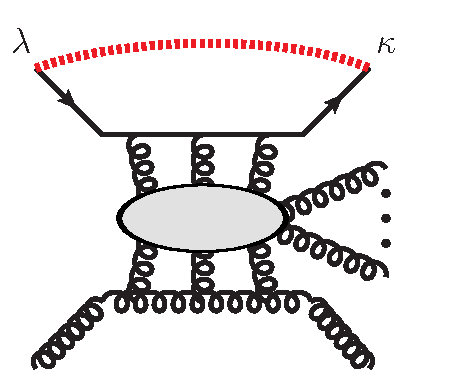
\includegraphics[scale=0.5]
    {figures/singleQuark.pdf}};
    % 5 point masters
    \node at (7,-.1){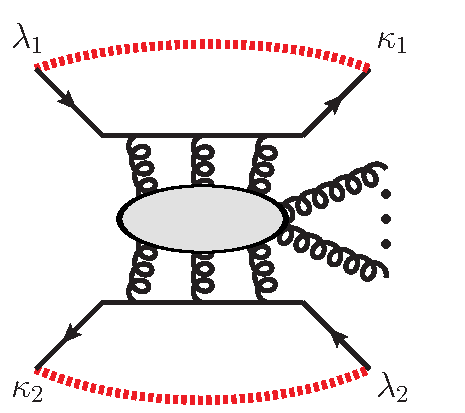
\includegraphics[scale=0.5]
    {figures/doubleTrace.pdf}};
\end{tikzpicture}
\end{center} 
\caption{Contraction of the open $(D_s-4)$-dimensional spinor indices for amplitudes
with external quarks: each quark line closes upon itself.
Indices connected by red dashed lines are traced over.}
\label{fig_traces}
\end{figure}
%%%%%%%%%%%%% FIGURE %%%%%%%%%%%%%%%%%%
\begin{figure}[]
  \begin{center}
  	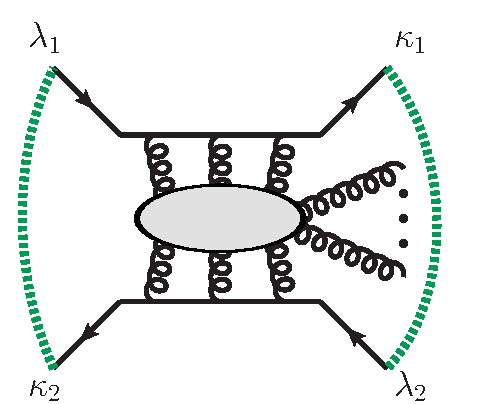
\includegraphics[scale=0.5]
    {figures/singleTrace.pdf}
\end{center} 
\caption{Alternative contraction of $(D_s-4)$-dimensional spinor indices leading to a
single trace. Indices connected by green dashed lines are traced
over.}
\label{fig_SingleTrace}
\end{figure}





\subsection{Chiral couplings ($\gamma_5$)}

\todo{do I really want this to be here\ldots?}

We emphasize that we do not invent regularization scheme thus there's nothing new we say about $\gamma_5$ issue.

At least general remarks should be written 

One clearer insight is that inconsistent algebras cannot be applied here due to non-analyticity.
So the only consistent method should be when $\gamma_5$ commutes with higher dim. matrices.


\subsection{Discussion}
\label{sec:dshel_discussion}

\todo{Validated extremely well by reproducing all the results computed from the form-factor decomposition} 

\todo{Important transition between schemes} 
The two schemes are consistent,
in that their contributions to NNLO computations can be related by known
transition rules~\cite{Broggio:2015dga}, but as we
shall see below the HV scheme introduces some simplification in
the calculation.

The idea of embedding external states into higher-dimensional spaces to obtain
helicity amplitudes in dimensional regularization is not new. 
It has been employed in one-loop numerical generalized
unitary methods \cite{Ellis:2007br,Giele:2008ve}, as well as as 
the so-called six-dimensional helicity formalism \cite{Bern2011,Cheung:2009dc,Badger:2013gxa,Badger:2017jhb} for two loops.
However the embedding of fermionic states, in particular any number of them,
and the relation to the HV scheme were largely glossed over,
which caused some confusion in the past.

For example if one takes a ``single'' embedding of external quarks \todo{expand on this, reference an explicit state} ,
one effectively considers an amplitude polarized in $\mathsf{S}_{[D_s-4]}$ \todo{unify space names},
so the computation carried out in this way do not correspond to the HV scheme.
Strictly speaking then the arguments we used for the dimension of embedding of loop momenta are invalidated.

At the integrand level this manifests itself as appearing of explicit components of $\ell^\mu_{i[D-4]}$, not as scalar products $\mu_{ij}$ (see \cref{sec:PartialFractions}).
At one loop this was observed as ``odd $\mu$ powers'' in \cite{Fazio:2014xea,Badger:2017gta}.
It can be shown that if there are less than two \emph{massive} quark pairs, simply discarding 
the odd $\mu$ powers leads to the HV results to $\order{\eps^0}$.
However the differences will appear starting from $\order{\epsilon}$ for any amplitude
with more than two quark pairs, massive or not.
From two-loop onwards the differences will appear already in the poles in $\epsilon$. 
For example the single embedding was used in \cite{DeFreitas:2004kmi} for the computation of two-loop four-quark amplitudes,
and the result for the amplitude differs significantly from our results and the result of \cite{Glover:2004si}.
In \cref{sec:relevant_tensors} we explained why the finite remainders agree.

\todo{All particles can be massive, nothing changes, but the little-group scaling is replaced by the q-helicity scaling.} 


 

\section{$D_s$-Dependence From Dimensional Reduction}
\label{sec:ds_reduction}
Here we explain how to improve the extraction of $D_s$-dependence.
This is crucial for amplitudes with external fermions due to the exponential scaling of the representation.


The amplitudes $A$ defined in eq.~\eqref{eq:defAmpsTens} are polynomials in $D_s$,
\begin{equation}
  A(D_s) = \sum_{i=0}^{N} \mathcal{K}_i~D_s^{i}\ ,
  \label{eq:ds-poly}
\end{equation}
where $N$, the maximal power of $D_s$, 
varies depending on the process, the loop order, and the choice of tensor structure 
in eq.~\eqref{eq:tensorDecomposition}.
For the amplitudes considered in this paper $N\leq2$.
In this section we will suppress all arguments of $A$ and only keep track of the 
dependence on~$D_s$.
%
In a numerical framework, $A(D_s)$ can only be evaluated for integer $D_s$ values for which 
the particle states are well defined.
To be able to set $D_s=4-2\epsilon$ in the HV scheme, the knowledge of the coefficients $\mathcal{K}_i$ is required.
One way to obtain them is to reconstruct the polynomial \eqref{eq:ds-poly} from
a sample of $(N+1)$ integer values of $D_s$.
This procedure is known as dimensional reconstruction \cite{Giele:2008ve} and has  previously been applied
in \cite{Ellis:2008ir,Boughezal:2011br,Abreu:2017xsl,Abreu:2017hqn}.

While being generic and straightforward to implement, this approach has drawbacks which
become particularly evident in amplitudes with fermions.
%
The dimension of the spinor representation scales exponentially (as $2^{D_s/2}$) with $D_s$,
as opposed to the linear scaling of the vector representation.
Furthermore, the external spinor states with definite helicity can be embedded consistently
only for even values of $D_s$,
which pushes the sample values higher compared to the case of vector particles in the loops.
Beyond the obvious detrimental effect on the numerical complexity, the dimensionality of the
spinor representation determines the number of terms entering the evaluation of the traces
to obtain the helicity amplitudes through  eq.~\eqref{eq:defAmpsTens}. For
the case of amplitudes with multiple external quark pairs this makes the computation
of traces unnecessarily time consuming.

These considerations motivate the search for more efficient alternatives to dimensional
reconstruction. Here we employ one such alternative, based on the idea of
dimensional reduction, which has recently been presented in ref.~\cite{Anger:2018ove} 
and already applied to the computation of one-loop amplitudes in ref.~\cite{Anger:2017glm}.
In the remainder of this section we give a brief overview of this method 
and refer the reader to ref.~\cite{Anger:2018ove} for more technical details.

We start by rearranging eq.~\eqref{eq:ds-poly} in the following way:
\begin{equation}
  A(D_s) = \sum_{i=0}^{N} \tilde{\mathcal{K}}_i~(D_s-D_0)^{i},
  \label{eq:ds-poly-alt}
\end{equation}
where $D_0$ is some \textit{base} dimension, and the coefficients $\tilde{\mathcal{K}}_i$
can be obtained by a linear transformation of the coefficients $\mathcal{K}_i$ in eq.~\eqref{eq:ds-poly}.
It turns out that, given a suitable choice of $D_0$,
the dependence of $A(D_s)$ on degrees of freedom higher than $D_0$ can
be captured in a kinematic-independent way.  
This observation allows one to analytically separate this
dependence, and thus evaluate each coefficient $\tilde{\mathcal{K}}_i$
directly. Furthermore, these evaluations are then performed in the base
dimension $D_0$, resulting in spinor representations of much lower dimensionality
compared to those encountered in the framework of dimensional reconstruction.

For reasons that will become clear shortly, one chooses the base
dimension $D_0$ to be the minimal dimension which allows to embed 
all loop-momentum components without introducing new relations.
For two-loop amplitudes we have $D_0=6$, and we
shall specialize to this case henceforth. We write the metric tensor as
a direct sum,
  \begin{align}
    \label{eq:ds-split-metric}
    g^{\mu\nu}_{[D_s]}  = g^{\mu\nu}_{[D_s-6]} + g^{\mu\nu}_{[6]},  \qquad
    g^{\mu\nu}_{[D_s-6]}g^{\phantom{\mu\nu}}_{\mu\nu\,[6]} = 0\,,
  \end{align}
  and the gamma matrices as a direct product 
  (see e.g.\ \cite{Collins:1984xc,Kreuzer:susylectures}),
\begin{equation}
  (\gamma_{[D_s]}^\mu)_{a\kappa}^{\,b\lambda}  = \left\{ 
    \begin{array}{ll} 
      \left(\gamma_{[6]}^\mu\right)_a^{\;b} \,
      \delta_\kappa^\lambda\,, &\quad  0\le\mu \le 5 \,,\\&\\
      \left(\gamma^\star_{[6]}\right)_a^{\;b} 
      \left(\gamma_{[D_s-6]}^{(\mu-6)}\right)_\kappa^{\;\lambda}\,, 
      &\quad \mu \geq 6 \,,
    \end{array}
    \right.
    \label{eq:ds-gamma}
\end{equation}
where $\gamma^\star_{[6]}$ is a six-dimensional analogue of $\gamma_5$ in four dimensions, i.e.\ $\{\gamma^\star_{[6]},\gamma_{[6]}^\mu\} = 0$ for all $\mu \in \{0,5\}$, and $(\gamma^\star_{[6]})^2 = 1$.
The product representation allows us to factorize any chain of gamma matrices into a product of $6$- and $D_s-6$-dimensional gamma-matrix chains.
Then, using the fact that the trace of a direct product of two matrices is the product of their traces,
we can split the traces required to obtain the coefficients of tensor structures in eq.~\eqref{eq:tensorDecomposition}
as follows:
\begin{equation}
  \Tr\left(\prod_{\mu_i\in \mathcal{G}}\gamma^{\mu_i}_{[D_s]}\right) =
  \Tr\left(\prod_{\mu_i\in \tilde{\mathcal{G}}}\gamma^{\mu_i}_{[D_s-6]}\right) \cdot
  \Tr\left(\prod_{\mu_i\in \mathcal{G}}\gamma^{\mathfrak{I}(\mu_i)}_{[6]}\right),
  \label{eq:ds-split-traces}
\end{equation}
where the product on the left-hand side is over a sequence $\mathcal{G}$ of $D_s$-dimensional Lorentz indices,
$\tilde{\mathcal{G}} = \{ \mu_i \in \mathcal{G} ~\vert~ \mu_i \geq 6 \}$, and the map $\mathfrak{I}$ is defined as
\begin{equation}
  \mathfrak{I} : \mu \to
    \begin{cases}
      \mu, & 0\le\mu \le 5\,, \\
      \star, & \mu \geq 6\,.
    \end{cases}
\end{equation}
The traces of $\prod_{\mu_i\in\tilde{\mathcal{G}}}\gamma^{\mu_i}_{[D_s-6]}$ can be 
evaluated analytically using well-known Clifford algebra identities,
which produce sums of products of $g^{\mu_i\mu_j}_{[D_s-6]}$.
%
The crucial observation is that the only object to be contracted with the indices beyond 
$(D_s-6)$ is $g^{\mu\nu}_{[D_s-6]}$.
This is ensured by our choice of the base dimension.
These indices then always contribute terms of the form $g^\mu_{[D_s-6]\mu} = (D_s-6)$, 
generating contributions to the coefficients $\tilde{\mathcal{K}}_i$ with $i>0$ 
in eq.~\eqref{eq:ds-poly-alt}. At this point, all degrees of freedom beyond $(D_s-6)$
are traded for polynomials in $(D_s-6)$ with integer factors, and the coefficients
$\tilde{\mathcal{K}}_i$ are expressed in terms of six-dimensional objects only.

\todo{Put examples of tree and 1-loop.}

\subsection{Dimensionally Reduced Feynman Rules}
\label{sec:DsFeynRules}
In the table~\ref{tab:Ds-FeynRules} we list the color-ordered Feynman rules for vertices involving the scalar particles introduced in section~\ref{sec:Ds}.
The $(D_s-6)$-dimensional part of these rules can be fully contracted in each Feynman diagram yielding kinematic-independent factors.
\begin{table}[h]
  \centering
  \begin{minipage}[t]{0.4\textwidth}
    \small
  \begin{tabular}{cl}
    $\vcenter{\hbox{\hspace{-2ex}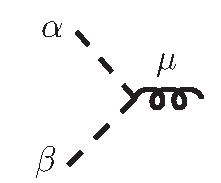
\includegraphics[width=13ex]{figures/Vssg}}}$ & $ \frac{i}{\sqrt{2}}(p_2-p_1)^\mu~ g^{\alpha\beta}_{[D_s-6]}$ \\
    $\vcenter{\hbox{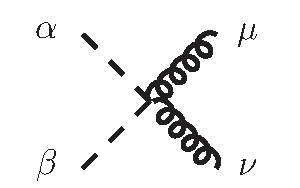
\includegraphics[width=15ex]{figures/Vssgg}}}$ & $ -\frac{i}{2}~g^{\mu\nu}_{[6]}~g^{\alpha\beta}_{[D_s-6]}$ \\
    $\vcenter{\hbox{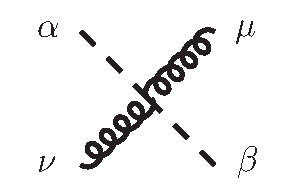
\includegraphics[width=15ex]{figures/Vsgsg}}}$ & $ i~g^{\mu\nu}_{[6]}~g^{\alpha\beta}_{[D_s-6]}$ \\
  \end{tabular}
  \end{minipage}
  \quad
  \begin{minipage}[t]{0.5\textwidth}
    \small
  \begin{tabular}{cl}
    $\vcenter{\hbox{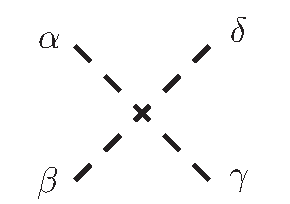
\includegraphics[width=15ex]{figures/Vssss1}}}$ &
      $
      \begin{aligned}
        i~g^{\alpha\gamma}_{[D_s-6]} g^{\beta\delta}_{[D_s-6]} - ~ & \\
                \frac{i}{2}~(g^{\alpha\beta}_{[D_s-6]} g^{\gamma\delta}_{[D_s-6]} & + g^{\alpha\delta}_{[D_s-6]} g^{\beta\gamma}_{[D_s-6]})
      \end{aligned}
      $ \\
        $\vcenter{\hbox{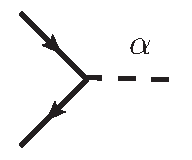
\includegraphics[width=11ex]{figures/VqqsR}}}$ & $- \frac{i}{\sqrt{2}}~\gamma^\star_{[6]} \gamma^\alpha_{[D_s-6]}$ \\
        $\vcenter{\hbox{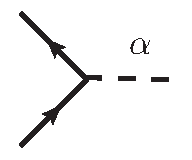
\includegraphics[width=11ex]{figures/VqqsL}}}$ & $ \frac{i}{\sqrt{2}}~\gamma^\star_{[6]} \gamma^\alpha_{[D_s-6]}$ \\
  \end{tabular}
  \end{minipage}
  \caption{Color-ordered Feynman rules for vertices with scalar particles explicitly introduced by dimensional reduction of gluons.}
  \label{tab:Ds-FeynRules}
\end{table}

\FloatBarrier

From a Feynman diagrammatic perspective, the contributions to the
coefficients of the polynomial in $(D_s-6)$
can be represented by introducing a scalar particle. 
The Feynman rules associated to this particle can be readily
derived from dimensional reduction of the original Feynman rules of the
theory \cite{Bern:2002zk,Badger:2013gxa,Giele:2008ve,Anger:2018ove} by
applying the relations \eqref{eq:ds-split-metric} and \eqref{eq:ds-gamma}.
We list them in the appendix \ref{sec:DsFeynRules} for convenience.
To illustrate this procedure we now give an example. 
Consider a decomposition of a Feynman diagram with $D_s$-dimensional particles on the 
left-hand side of figure~\ref{fig:ds-example-diagram}. The four non-vanishing 
contributions after evaluating partial traces and contracting all 
$(D_s-6)$-dimensional indices are shown on the right-hand side, 
where the scalars are introduced to represent what remains of these contractions.

\begin{figure}
  \newlength\diagramWidth
  \setlength{\diagramWidth}{18ex}
  \centering
  \begin{align*}
    \vcenter{\hbox{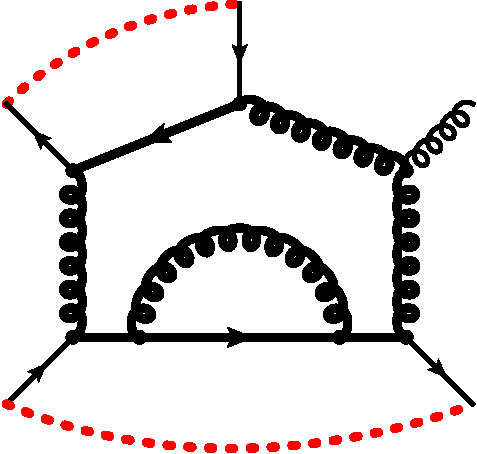
\includegraphics[width=\diagramWidth]{figures/Ds-example_B.pdf}}} \hspace{-10ex} & \hspace{15ex} = \hspace{6ex}
    \vcenter{\hbox{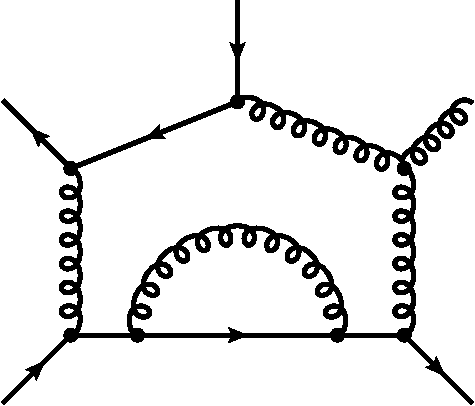
\includegraphics[width=\diagramWidth]{figures/Ds-example.pdf}}} \quad +\\
    \Big(~ &
    \vcenter{\hbox{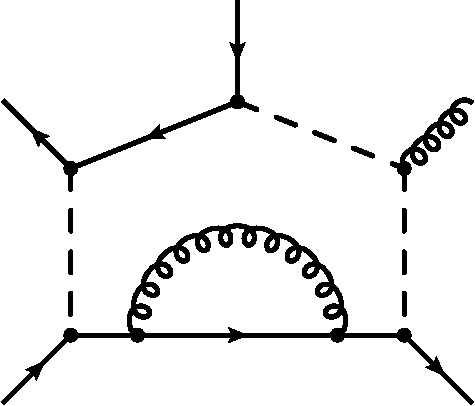
\includegraphics[width=\diagramWidth]{figures/Ds-example-1-1.pdf}}} \quad+\quad
    \vcenter{\hbox{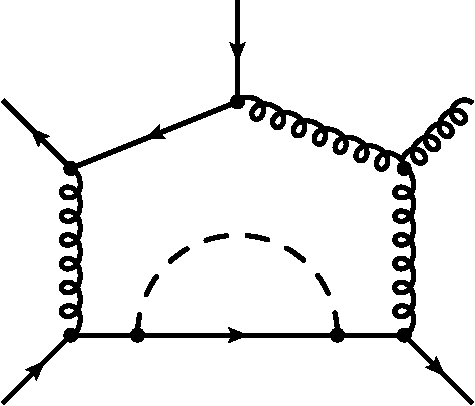
\includegraphics[width=\diagramWidth]{figures/Ds-example-1-2.pdf}}}
    ~\Big) ~\cdot~ (D_s-6) \quad +\\
    &
    \vcenter{\hbox{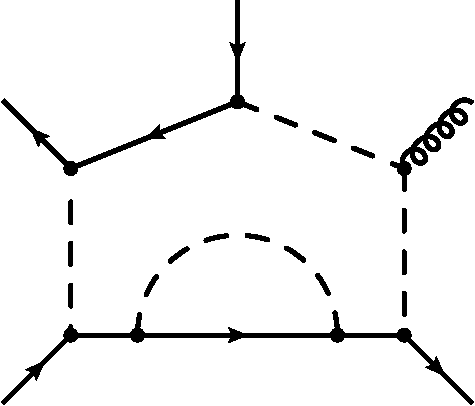
\includegraphics[width=\diagramWidth]{figures/Ds-example-2.pdf}}}
    ~\cdot~ (D_s-6)^2,
  \end{align*}
  \caption{Example of diagrams with scalar particles,
    representing the contributions to the coefficients of $\tilde{\mathcal{K}}_i$ in eq.~\eqref{eq:ds-poly-alt}.
    The thick lines in the diagram on the left-hand side represent particles in arbitrary $D_s$ dimensions.
    The (red) dashed lines connecting external-quark lines represent the traces required to obtain the coefficient of the tensor structure of eq.~\eqref{eq:defAmpsTensb}.
    All particles on the right-hand side are in six dimensions.}
  \label{fig:ds-example-diagram}
\end{figure}


We would like to conclude this section with some remarks.
First, the remaining non-trivial traces of eq.~\eqref{eq:ds-split-traces},
i.e.\ those of $\prod_k\gamma^{\mu_k}_{[6]}$, cannot be simplified generically
as the indices appear contracted with the loop momenta at the integrand level.
We evaluate them by the direct summation over a specially constructed set of external states
(in an analogous way to the sums performed in~\cite{Abreu:2018jgq} 
for dimensional reconstruction).
Secondly, in the absence of fermions in the loops, this method coincides with the so called
six-dimensional formalism employed in refs.~\cite{Badger:2013gxa,Badger:2017jhb}, and can 
thus be viewed as an extension thereof to amplitudes with fermions.
Finally, we note that the method presented in this section can be straightforwardly
generalized to higher number of loops by adjusting the base dimension $D_0$,
as well as to the extraction of coefficients of different tensor structures in 
eq.~\eqref{eq:tensorDecomposition}.



\subsection{Unitarity-Compatible Implementation}
decomposition of trees through simplified off-shell recursion.
    Collecting $(D_s-6)$ powers and factors. Implementation in process libraries.

    \todo{Use tree example here}



